%!TEX TS-program = xelatex
%!TEX encoding = UTF-8 Unicode

\documentclass[12pt]{report}
\usepackage[vmargin = 3cm]{geometry}
\linespread{1.25}
\geometry{a4paper}
\usepackage{enumitem}
\usepackage{url}
\usepackage{fontspec,xltxtra,xunicode}
\usepackage{amsmath}
\defaultfontfeatures{Mapping=tex-text}
\setromanfont[Mapping=tex-text]{Linux Libertine O}

%Code Hilighting
\usepackage{minted}
\usemintedstyle{friendly}
\newminted{objc}{fontsize=\footnotesize}

%Graphics shit
\usepackage{graphicx}
\DeclareGraphicsExtensions{.pdf,.png,.jpg}

%Bibliography
\usepackage{biblatex}
\bibliography{references}

\title{Location Aware Reminders for iOS\\ \small{Supervised by Russell Beale}}
\author{Alex Layton - 1080395}
\date{11 April, 2013}

\begin{document}

\maketitle

\begin{abstract}

Mobile apps have become increasingly popular with the rise of various mobile operating systems and their respective app stores. These app stores allow users access to a multitude of apps from utilities to games, and as the capabilities of these phones increase they allow more complex apps to be built using the sensors built into the device. A popular mobile operating system is Apple's iOS, which was updated in iOS5 to include a Reminders app. This app features the ability to add geo-fenced location reminders which alerts the user when they are in the specified location. These geo-fenced reminders have few uses, whereas a reminder which could preempt when to alert the user based on their current location and their destination has a wide range of uses.\\

This report looks into the design and implementation of preemptive reminders as well as the process of creating an app for the App Store.

\end{abstract}

\tableofcontents
\newpage

\chapter{Introduction}

\section{Motivation}

With the increasing popularity of mobile devices their are more opportunities to create mobile apps which can be distributed through various app stores on a number of mobile operating systems. The operating systems boast millions of users, which collectively download billions of apps from the hundreds of thousands available on their devices app store. Consider Apple's iPhone, which runs iOS. Their latest version of iOS - iOS6 has around 300 million users and their App Store offers over 800,000 apps that have been downloaded a total of 4 billion times \cite{applenumbers}. This shows what a great opportunity these app stores are and allow smaller developers to distribute their app on a scale thats usually only seen by larger developers. Although their is the possibility of mass user adoption, it is also easy to go unnoticed amongst the other hundreds of thousands of apps.\\

As the adoption of these devices increases they are being used to complete more and more tasks. These tasks can be important such as calendaring in order to allow the user to organise their time or setting alarms and reminders. Traditionally a reminder simply alerts the user at a set time with the given reminder. As the capabilities of mobile devices have increased and the introduction of GPS and GLONASS \footnote{Global Navigation Satellite System} sensors have allowed reminders to make use of location data, which can be seen in Apple's Reminders app where instead of a reminder being triggered by a time it is triggered by a location, specifically when the users current location is within a certain distance from the desired location. This technique is known as geo-fencing \cite{geofence} and is essentially creating a virtual perimeter around a location so once that area is entered a task can be performed, whether it is downloading something in the background or in this case alerting the user with a reminder. The problem with these geo-fenced reminders is that they do not take time into consideration and as a result are limited in scope - a better solution would be one that considers both location and time.\\

By taking into account both location and time these reminders could be used to remind the user dependant on how far away they are from their destination and how long until they need to be there. For instance, if a user set a reminder for half an hour in the future, and it takes 15 minutes to reach that destination, providing the user doesn't move they should be alerted in 15 minutes in order for them to reach their destination on time. The scope of this functionality is much greater than the previously mentioned geo-fenced reminders, which could be used in any application that involves the user reaching a destination before a deadline. This project looks at the implementation of these reminders in the form of an iOS app.\\

\section{Aims}

There are several aims involved in this project. First and foremost the main aim of this is to implement the preemptive reminder functionality in an iOS app. The other main aim is to release the proposed functionality in an app available on the App Store. Another aim of the project is to create the preemptive reminder functionality as a library which would allow for other apps to easily make use of these reminders. Since using location services on a device can drastically drain the battery an aim is to try and make the app as efficient as possible by only using location when needed and using these services in a low power mode if possible. The created app to demonstrate the reminders functionality should also have a good user interface, as well as good user experience when adding location reminders.

\chapter{Analysis}

\section{Existing Apps}

It is important to research existing apps when building an app for a mobile device. As previously mentioned, with hundreds of thousands of apps available on the various distribution channels there is the possibility that the proposed functionality has already been implemented. By looking on the different app stores  its possible to see what applications are already available. The  mobile platforms with the biggest user bases are iOS and Android so its logical to target their respective stores - the App Store \cite{appstore} and the Google Play Store \cite{playstore} as the basis for researching existing apps.\\

On iOS there exists the previously mentioned Reminders app, which features the geo-fenced reminders functionality. Another app available on the app store is Checkmark \cite{checkmark}. This app builds upon the functionality in Reminders by allowing the user to set the radius of the geo-fence around a location as well as allowing the user to set a timer to alert them a specified amount of time after reaching the geo-fenced area. Geo-Reminders \cite{tapone} is another app that offers geo-fenced reminders.\\

For Android the existing apps are very similar in functionality to the ones available on iOS. Milwus Location Alarm \cite{milwus} is an example of geo-fenced reminders.\\

From the research conducted into existing apps, there are currently no apps that make use of the proposed functionality.\\

\section{Objective-C}

In order to build an iOS app an understanding of the Objective-C programming language is required. The language builds upon the C language by adding object-oriented patterns. It allows for method and classes as found in other objected-oriented languages while making use of core C APIs. As this report will cover the implementation of an app, it may be useful to demonstrate some parts of the Objective-C language.\\

\begin{figure}[H]
\begin{objccode}
#import <Foundation/Foundation.h>

@interface HelloWorld : NSObject
+ (void)hello1;
- (void)hello2;
@end

@implementation HelloWorld
+ (void)hello1 
{
    NSLog(@"Hello, World");
}
- (void)hello2 
{
    NSLog(@"Hello, World");
}
@end

int main(void) 
{
    [HelloWorld hello1];
    HelloWorld *hw = [[HelloWorld alloc] init];
    [hw hello2];
}
\end{objccode}
\caption{An Objective-C class demonstrating method calls}
\label{fig:helloworld}
\end{figure}

All Objective-C classes have an interface, this is where all the public methods are declared for that class. The method 'hello1' is declared with a '+' which shows that it is a class method, while 'hello2' declared with a '-' is an instance method. In this example the interface is declared inline, but it is more common to find a '.h' file for the interface while the implementation is found in a '.m' file.\\ 

The implementation for both of the methods is straight forward, with them both printing 'Hello, World'. You may notice that the function to print the string is prefixed with 'NS' as well as the class we are inheriting from. This is due to the fact that all classes within the Foundation framework were created for the NextStep platform and as a result still carry the naming convention from this platform. Class prefixes are common in Objective-C for instance the framework for user interfaces on iOS is called 'UIKit' and as a result all classes in this framework being with 'UI'. This project will include similar prefixing of class names.\\

Like other programming languages the main method is where the code is executed. Method calls in Objective-C are wrapped in square brackets, with the first word inside the bracket being the class and the second being the method call. As you can see, since 'hello1' is a class method the class does not need to be instantiated while the call to 'hello2' requires the class to be allocated memory and initialised.\\

Delegation is a widely used programming pattern within Objective-C. Since delegation will be used throughout the project it may also be useful to introduce this concept. According to the Apple Developer Documentation \cite{delegates}, a delegate is an object that acts on the behalf of another object in order to respond to an event received by this other object. For example, a class may hold an instance of a text field (UITextField) and the class may wish to be notified when the user presses the enter key on their keyboard, so the application  can behave accordingly. The documentation shows that the text field has a protocol reference - UITextFieldDelegate and that the textfield has a property called delegate that can be any object that subscribes to this delegate protocol. In order for the class that has the text field to be notified it should set the delegate property of the text field as itself and implement the following delegate method;

\begin{objccode}
- (BOOL)textFieldShouldReturn:(UITextField *)textField 
\end{objccode}

This means that now whenever the enter button is pressed while using the text field, the text field instance calls the above method on the instance that is stored in the delegate property. A better example of delegation is;

\begin{figure}[H]
\begin{objccode}
@protocol ADelegate <NSObject>
- (void)aDelegateMethod;
@end

@interface A : NSObject {}
@property id<ADelegate> delegate;
- (void)start;
@end

@implementation A
- (void)start
{
    //do something here then call
    if (_delegate) [_delegate aDelegateMethod];
}
@end

@interface B : NSObject <ADelegate>
@property A *a;
- (void)run;
@end

@implementation B
- (void)run
{
    _a = [[A alloc] init];
    _a.delegate = self; //we are a's delegate
    [_a start]; //call aDelegateMethod when something happens
}
- (void)aDelegateMethod
{
    NSLog(@"Hello, World");
}
@end

int main(void) 
{
    B *b = [[B alloc] init];
    [b run];
}
\end{objccode}
\caption{Objective-C class to demonstrate setting a delegate}
\label{fig:delegation}
\end{figure}

From the above example you can see there is a protocol declaration. This is where the delegate methods are declared. 

The tools to write and run Objective-C code are freely available and developers can install the Xcode IDE which provides a toolchain to allow Objective-C code to be compile, run (or simulated), tested and profiled. Xcode requires a machine running Mac OS X, but Objective-C code can be compiled on any machine that can run the llvm compiler. In order for developers to release their apps on the App Store, they must be provisioned and submitted to Apple for approval. An Apple developers license is required in order to do this.

\section{Data Sources}\label{sec:datasources}

As this project will require location data in order for the user to find both places of interest as well as searching for places there needs to be a data source that is useable within this project. By using a web services API it would provide a number of benefits including the fact that that the data used does not need to be stored on the device as the service provider manages the data. However there are several drawbacks to using a web API especially on a mobile device. As these APIs are accessed over the web, an internet connection is necessary in order to make requests but is sometimes the case that a device may not have the signal to make these requests. Another drawback is that if the provider is experiencing problems and an API that is being used is unavailable it could result in a large component of the app not working.\\

In terms of location data two providers have been identified, as Google and Foursquare. Google provides a Places API \cite{placesapi} that returns places of interest around a given location. It also allows for a search query to be given which will then return nearby places that match the search term. When using this API the output can be specified as JSON\footnote{JavaScript Object Notation} or XML\footnote{Extensible Markup Language}. XML is a popular choice for representing data on the web, but JSON provides an alternative that is more human readable and a large number of parsers exist for this notation on iOS \cite{json}. Foursquare provides a similar service to Google's Places API known as their Venues Platform \cite{foursquare}. As with Google's API the data is returned as JSON so can be parsed in the same way. Google also offer a Geocoding API \cite{geocodingapi} which may also be useful in this project. Geocoding is the process of taking a location and turning it into an address. This API can take a location in the format of a latitude and longitude and output the address as JSON. This functionality may not be beneficial, but Google also provide the ability to reverse geocode. This would allow for the implementation of a search feature where the search query could be used as the address which is to be reverse geocoded and then resulting location could then be used. 

\section{Literature Review}

The Apple Developer Center \cite{devcenter} provided much of the necessary information to enable the implementation of this project. This website provides all the necessary documentation to use Apple provided frameworks as well as presentations from developer conferences introducing newly implemented functionality in frameworks and new features in the iOS operating system. Apple also provide example implementations in order to demonstrate presented functionality.

Since the proposed reminder functionality requires location it was important to research into the existing location frameworks and APIs available on iOS. The WWDC presentation - 'Staying on Track with Location Services' \cite{locationservices} provides a good high level insight into the location technologies used within iOS. This presentation identified several factors needed for the implementation of location reminders. One of these factors is background execution, since reminders are essentially useless if the app can only be run in the foreground. In order to be allowed to execute in the background the app needs to register as an app that can run in the background. The presentation demonstrates how to register as a background app by adding the XML code in Figure \ref{fig:plist} to the apps \texttt{Info.plist} file.

\begin{figure}[h!]
\begin{minted}{html}
<key>UIBackgroundModes</key>
<array>
<string>location</string>
</array>
<key>Required background modes</key>
<array>
<string>Appregistersforlocationupdates</string>
</array>
\end{minted}
\label{fig:plist}
\caption{plist code required for the app to run in the background}
\end{figure}

Although it is possible to run standard location services while in the background, there exists methods within the CoreLocation framework to allow for monitoring of significant changes. These significant location changes make use of cell tower triangulation instead of wi-fi, GPS and GLONASS which is used my the standard location changes.

TODO: Add section on delegation to objective c and then talk about location update thingy

Another factor in this project is using maps. Since reminders will use location, using maps will provide a way to give user specified locations context. Apple also provide a MapKit presentation from their WWDC sessions called; 'Getting Around Using MapKit' \cite{mapkit}. This presentation introduces the new maps released in iOS6 as well as how to implement them into an app. Since MapKit uses the CoreLocation framework itself in order to show the users current location on a map, it is easy  to use the two frameworks together.

Storyboards provide an alternative way to create user interfaces and were originally introduced with iOS5. This method differs to traditionally used methods to design iOS app such as using NIB \footnote{NeXT Interface Builder} files and creating the interface completely programatically. The WWDC presentation - 'Adopting Storyboards in your app' \cite{storyboards} provides insight into how to transition from older interface building methods to the newer Storyboards. Pennington states that there are two main concepts involved with Storyboards, one being scenes and the other segues. The scenes are the view controllers that will display the different views in the application, while segues are the connections and transitions between scenes. (show an image with of storyboard)

These storyboards are created graphically, which are then connected to code by specifying a scenes class. For instance a UIViewController could be dragged onto the storyboard, with a class existing called MyViewController that subclasses UIViewController. This subclass can then be set as that scenes class so when the scene is displayed it instantiates that class as opposed to using a standard UIViewController. Segues are also created graphically by dragging an arrow from a user interface element to a destination scene. Segues can be detected programmatically in order to react to the transition, for instance data can be passed to the destination view controller or data could be saved before the view changes. Since a view could have multiple segues to different destinations, a segue can be given an identifier so that it is possible to detect not only the segue but the destination of that segue. The following method is called in a UIViewController subclass when a segue is about to happen;

\begin{minted}{objc}
- (void)prepareForSegue:(UIStoryboardSegue *)segue sender:(id)sender
\end{minted}

This method takes a segue object and a sender. The sender is the object where the transition is initiated, so if the segue is occurring because of a button press, the sender will be the UIButton that was pressed. The class reference for UIStoryboardSegue \cite{segue} shows that it contains a properties for the destination view controller and an identifier. The destination view controller is an an instance of the view that will be displayed to the user, this allows properties of the destination view controller to be set before it is shown to the user. The identifier, like previously mentioned contains the string of the identifier given for that segue.

Since the app will use a custom interface it is important to research how to create an interface using the non standard UI elements available. Apple's WWDC talk on 'Advanced Appearance Customization on iOS' \cite{appearanceios} demonstrates techniques in order to customise the user interface of an app. The presentation shows that all custom interface elements should be images created at the correct size for the device it is being used on. For instance an image created for a device such as the iPhone 3GS could be called 'myImage.png', while the image for a device such as the iPhone 4 should be called 'myImage@2x.png' and should be twice as big as the original image to account for the increased pixel density of the device. Once the images are named correctly they can be instantiated programmatically simply from the following line of code;

\begin{minted}{objc}
UIImage *myImage = [UIImage imageNamed:@"myImage"];
\end{minted}

The presentation also goes on to demonstrate using resizable images as opposed to fixed width ones. One use for resizable images is buttons. Since it is common to have multiple buttons, each with there own text, a resizable image would allow the button to change size depending on the length of text. This is not the case for a button using a fixed width image and the resulting button might be using an image that is much bigger than the text the button holds. Figure \ref{fig:resizableimage} demonstrates creating a button from a resizable image.

\begin{figure}[h!]
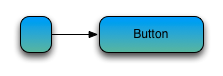
\includegraphics[scale=0.75]{images/resize-image}
\begin{objccode}
    UIImage *myImage = [UIImage imageNamed:@"myImage.png"];
    //first 15 pixels and last 15 pixels across aren't resizable
    UIEdgeInsets insets = UIEdgeInsetsMake(0, 15, 0, 15)
    UIImage *buttonImage = [myImage resizableImageWithCapInsets:insets];
    UIButton *myButton = [[UIButton alloc] init];
    [myButton setTitle:@"Button" forState:UIControlStateNormal];
    [myButton setBackgroundImage:buttonImage forState:UIControlStateNormal];
\end{objccode}
\label{fig:resizableimage}
\caption{Code to demonstrate resizable images in Objective-C}
\end{figure}


In order to customise the user interface as demonstrated above, the techniques described above would need to every instance of the UIKit objects used in throughout a project. As of iOS5, a UIAppearance property has been added to the various classes found within UIKit \cite{nshipster}. UIAppearance offers a way to style the different UI elements once and have them consistent throughout the app. UIAppearance is a protocol that classes in UIKit subscribe to. By calling the appearance class method of a UIKit class, an appearance proxy is returned. The appearance proxy is essentially an another instance of the same class that the appearance method is being called on. This proxy can be customised as if it were a normal object of that class type, but when an instance of that class is created it refers to the appearance instance to customise itself. An example may be a better way to demonstrate this functionality, as seen in Figure \ref{fig:uiappearance}.

\begin{figure}[h!]
\begin{objccode}
    UIImage *buttonImage = [UIImage imageNamed:@"buttonImage.png"];
    [[UIBarButtonItem appearance] setBackgroundImage:buttonImage
                                            forState:UIControlStateNormal
                                               style:UIBarButtonItemStyleBordered
                                          barMetrics:UIBarMetricsDefault];
    //This bar button should have buttonImage as background...
    UIBarButtonItem *barButton = [[UIBarButtonItem alloc] init];
\end{objccode}
\label{fig:uiappearance}
\caption{Code to demonstrate using a UIAppearance proxy}
\end{figure}

By using \texttt{UIAppearance} it means a lot less code is duplicated in order to create similar looking UI elements throughout the app. Although using this technique allows the majority of properties of \texttt{UIKit} classes to be customised it is not available for some properties, so it may be the case that some particular properties must be customised once instantiated \cite{gist}.

\section{Project Specification}

From researching existing apps and looking at current programming paradigms and techniques for the iOS platform it may be beneficial to look at the original project aims and redefine them based on this research.\\

The main aim of this project to implement the proposed reminders functionality. Since this will be an iOS app, this functionality will be implemented in Objective-C, making use of the researched frameworks and techniques. The location component of this app will make use of the CoreLocation framework, using standard location changes in the foreground in order to give the user accurate location data while using the app. Once the app is sent to the background it will transition to significant location change services in order to use as little power as possible. It should also be the case that location is only used when needed and not for the duration the app runs for whether this is in the background or foreground. In order to provide an intuitive interface the app will also use the functionality found in the MapKit framework in order to give the locations received from the location services and given as destinations context to the user. The app will also take advantage of Storyboards to create the user interface as not only will it allow for rapid development of the app, but it allows a clear distinction to be made between user interface and functionality when building the app. The design of the app must be unique while also being consistent to the design language used on the platform, this can be validated from user testing by receiving feedback about the design. The interface should also make use of the previously mentioned \texttt{UIAppearance} protocol in order to create custom yet consistent UI elements throughout.\\

There are also requirements not directly related to the implementation of the app. The first is that upon completion of building and testing the app, it should be made available for users to download on the App Store. This requirement can be validated by the app being submitted to Apple for review, passing review and being downloaded on a user's device.

\chapter{Project Specification MKII}

From researching existing apps and looking at current programming paradigms and techniques for the iOS platform it may be beneficial to look at the original project aims and redefine them based on this research.

\section{Functional Requirements}

Functional requirements cover what functionality must be implemented in the app. The functional requirements necessary to implement the proposed functionality are as follows;

\begin{enumerate}[label*=\arabic*.]

\item{Implement Reminders functionality in an app}
    \begin{enumerate}[label*=\arabic*.]
        \item{Date based reminders}
        \item{Geo-fenced location reminders}
        \item{Preemptive reminders using location and date}
    \end{enumerate}
    
\item{Use the CoreLocation framework to interact with the location services available for a users device}
    \begin{enumerate}[label*=\arabic*.]
        \item{Only use location when required}
        \item{Use the low power significant change location service when the app is operating in the background}
    \end{enumerate}
    
\item{Show users location and reminder destinations on a map}
    \begin{enumerate}[label*=\arabic*.]
        \item{Use mapping functionality from the \texttt{MapKit} framework}
        \item{Implement navigation to allow the user to navigate from their current location to a destination}
    \end{enumerate}
   
\item{Implement a system to allow for reminders to be added quickly and easily}
    \begin{enumerate}[label*=\arabic*.]
        \item{Use location data from a number of sources}
        \item{Implement navigation to allow the user to navigate from their current location to a destination}
    \end{enumerate}

\end{enumerate}

\section{Non Functional Requirements}

Non functional requirements are those that relate to the proposed app, but are not requirements that affect how the app works at an implementation level. The non functional requirements detailed here are based upon those from Somerville...

\subsection{Development}

\begin{enumerate}[label*=\arabic*.]

\item{The app should be implemented in the Objective-C programming language}

\end{enumerate}

\subsection{Usability}

\begin{enumerate}[label*=\arabic*.]

\item{The app should be intuitive and easy to use}
    \begin{enumerate}[label*=\arabic*.]
        \item{Navigation throughout the app should be obvious and simple}
        \item{Buttons should be appropriately labeled either showing suitable text or a recognisable icon}
    \end{enumerate}

\item{The user interface should be unique}       
    \begin{enumerate}[label*=\arabic*.]
        \item{The interface should still follow design guidelines on iOS}
        \item{Custom UI elements should be using the \texttt{UIAppearance} protocol to look consistent throughout the app}
    \end{enumerate}

\end{enumerate}

\subsection{Peformance}

\begin{enumerate}[label*=\arabic*.]

\item{The app should minimise battery usage throughout usage of the app}
     \begin{enumerate}[label*=\arabic*.]
        \item{Use low power location service settings}
        \item{Only use location services when necessary}
        \item{Only run the app in the background when needed}
    \end{enumerate}
    
\end{enumerate}

\subsection{Reliability}

\begin{enumerate}[label*=\arabic*.]

\item{Reminders should be persistent between uses of the app}
     \begin{enumerate}[label*=\arabic*.]
        \item{Reminders should be saved so that the can be reloaded if the app not in use and removed from the background}
        \item{Added reminders should not disappear without being used}
    \end{enumerate}
    
\end{enumerate}

\subsection{Security}

\begin{enumerate}[label*=\arabic*.]

\item{No personal data must be stored or transferred}
     \begin{enumerate}[label*=\arabic*.]
        \item{Only current location should be used with data providers}
        \item{All data transfer must be secured and sent over SSL}
    \end{enumerate}
    
\end{enumerate}

\subsection{Portability}

\begin{enumerate}[label*=\arabic*.]

\item{User should be able to run app on any iOS device with location services enabled}
     \begin{enumerate}[label*=\arabic*.]
        \item{iOS6 is required to make use of newer functionality in \texttt{Core Location}}
    \end{enumerate}
    
\end{enumerate}

\chapter{Design}

There are several considerations to take in the design of this application. The first and main consideration is how the functionality of the app should work, while the other design considerations actually involve the graphical design of the app. Since both the user interface an the user experience are important aspects of this project, they will both be covered in this section of the report.

\section{Reminder Functionality}

The initial idea for the preemptive location reminders was to implement them as a separate framework to the app which then could be imported and use, which would be that the reminder functionality could be added to other apps. In Objective-C programming, especially iOS programming a common paradigm is to have an object, a data store for that object and then a manager that manages the data store and allows for functions to be performed on that data as well as responding to events through delegation. This is evident in a framework such as \texttt{CoreLocation}, which provides a \texttt{CLLocation} object as the data, while a \texttt{CLLocationManager} is used to receive the location objects and provides delegation methods through its \\\texttt{CLLocationManagerDelegate} protocol. The proposed reminder functionality will follow not only the naming conventions used for these previously mentioned classes, but also following the implementation patterns.  

\subsection{Reminder}

The reminder needs to encapsulate all aspects of the reminder functionality that is to be implemented. At its core, a reminder needs to consist of a location which is the destination for the reminder and a date which is when the reminder should alert the user. It is also necessary to have a message or subject which can be displayed to the user when they are alerted in order to remind them. Since the app will also offer other times of reminder alongside the preemptive ones, it will also be useful to store the type of a reminder.

\subsection{Data Store}

The data store will allow for multiple reminders to be used and stored, so there are several factors that need to be considered with this store. Firstly since there will be multiple types of reminders, it may be useful to store them separately so that they can be easily listed in their individual reminder categories as well as the fact that each reminder type will be processed separately. Reminders should be stored in data order, this means that the reminder with the date closest to the current date should be looked at first. In order to store the data in this way the most ideal structure would be a priority queue \cite{priorityqueue}. The priority would be based on the reminder objects date, which as previously mentioned would be ordered by the date closest to now being at the top of the list. This would mean that processing would always take place on the first element in the list as the reminder in the second position in the queue will not need to be fired until the first position reminder has. By creating a data structure such as the one mentioned here, it will be less work to actually process the reminders as they are already in a format that can be used.\\

Another consideration is the storage of this data. In Objective-C in order to store data on disk, the classes that are to be stored need to subscribe to the \texttt{NSCoding} protocol \cite{nscoding}. A lot of the classes found in the \texttt{Foundation} framework are \texttt{NSCoding} compliant. These include; \texttt{NSArray}, \texttt{NSDictionary} as well as others such as \texttt{NSString}. By using a data structure from the \texttt{Foundation} framework it would allow data to be stored with little extra work as well as the performance gain from using an optimised data structure such as the ones mentioned above.

\subsection{Reminder Manager}

The reminder manager, much like \texttt{CLLocationManager} is where all of the processing will take place. Since this manager will be responsible for subscribing to location services it would be necessary to not only store a \texttt{CLLocationManager} class, but to also subscribe to its delegate protocol in order to be notified when the user moves to a new location. Referring back to the project specification, it is a requirement to only use GPS when necessary and as a result the location services will only be used when a location based reminder exists. If the user only has date based reminders stored then the location services will remain off until some form of location based reminder is added.\\

Since it is the reminder managers purpose to manage the reminders, the manager will store an instance of the previously mentioned data store. When a user adds a new reminder, the manager will receive it and in turn give it to the reminder store to place it in its priority list. The reminder manager will also be responsible for saving the reminder store to disk, using something such as \texttt{NSKeyedArchiver}, which would allow data to be stored in a key value format in a file on the disk. At instantiation of the reminder manager class \texttt{NSKeyedUnarchiver} could be used in order to read the saved reminders, creating persistent reminders between usages of the app, which is also another requirement mentioned in the project specification.\\

It will also be useful to allow users to add repeating reminders. Once a user is alerted about a reminder, before that reminder is removed a repeat property should be checked, if this property exists for a reminder it is re-scheduled for a new date, which is the original reminder date with an offset added to it dependent on how often the reminder should repeat. The new reminder can be added to the priority queue for that reminder type and the original reminder can be removed.\\

As there will be three types of reminders that the user can add, each reminder type will have to be processed differently, the following sections document the reminder manager will process each of these different types of reminder.

\subsubsection{Preemptive Reminders}

Preemptive reminders will be the most complex, so it is important to design an efficient system to process them. The reminder manager will receive location updates, so for each new location received from the \texttt{CLLocationManager} it will check the first reminder in the preemptive reminder priority queue. As these reminders will rely on distance, speed and time it will be useful to look at the following formula;

\begin{equation}
speed = \frac{distance}{time}
\end{equation}


In order to check whether the user needs to be alerted with the reminder, a number of steps need to be taken. Firstly we need to calculate the distance between the current location and the location of the reminder. Once the distance has been calculated, the next step is to establish the current speed of the user. In order to calculate the speed, we compare the current location with the last known location in order to get the distance between these two points. By using the \texttt{CLLocationManager}, the \texttt{CLLocation} object it returns contains a timestamp. Comparing the timestamps from the current and last known locations then allows us to calculate the time between them. Using the above formula allows us to work out the current speed of the user, using the calculated distance and time values. Now that we have a distance between the current location and the destination as well as the current speed of the user, we can rearrange the formula above to give us;

\begin{equation}
time = \frac{speed}{distance}
\end{equation}

Once we have how long it will take the user to reach their destination, we can add that amount of time to the current time to check that the estimated arrival time is before the time they wish to be reminded. If the time is after when they wish to be reminded, the user is alerted and shown the reminder.\\

A consideration to be made with the preemptive reminders is that they will only process reminders on a new location update. In order to get round this limitation a timer could be used, so that reminders are processed at regular intervals regardless of whether there is a location update. If the processing is handled by the timer, the last location update will be considered the users current location as well as using the last calculated speed of the user. Although the user is currently not moving, the assumption is made that they will travel at the same speed they were last moving.

\subsubsection{Location Reminders}

The location reminders or geo-fenced reminders will also require the location and a date in order to alert the user. Like preemptive reminders, the location ones will also process upon the user reaching a new location. Once a new location is received, an area will be created to check if the reminder destination is within this area. The date for the reminder is required in order to see if the user should be alerted on this day. The priority queue for the location reminders should be iterated through until a reminder is found that is not the current day. For each reminder processed the location of that reminder should be checked to see if it is within the area that was created. If the reminder is within that area, the user is alerted and the reminder is removed from the priority queue.

\subsubsection{Date Reminders}

Since date reminders do not require the user's current location, this reminder functionality will make use of timers to set when the user should be alerted. These can be scheduled once the reminder has been added and requires no further processing until the user has been alerted. These reminders should also be stored in their own priority queue, so that they can be displayed to the user when they wish to see what date based reminder they have scheduled. Once the user is alerted the reminder can be removed from the priority queue.

\section{App}

The app is where the reminder functionality will be integrated and provide a way to for the user to interact with this functionality. There will be several components to the app. These will include;

\begin{enumerate}[label*=\arabic*.]

\item{Reminder Lists}
\item{Adding Reminders}
\item{Reminders map}
\item{App settings}
    
\end{enumerate}

Each of these components will have a respective view that the user will be shown in the app. A basic diagram can be seen here in Figure \ref{fig:apphierarchy}, showing the hierarchical layout of the app.

\begin{figure}[H]
\centering
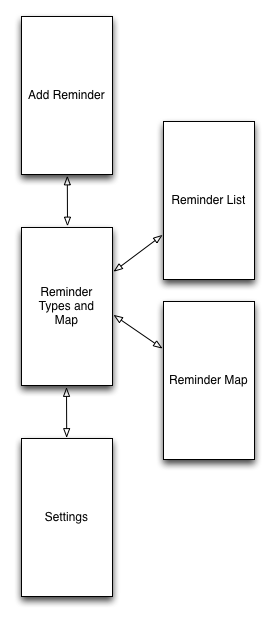
\includegraphics[scale=0.5]{images/app-hierarchy}
\caption{A diagram to show the hierarchical layout of the app}
\label{fig:apphierarchy}
\end{figure}

\subsection{Reminder Lists}

The reminder lists will contain all of the reminders for each type of reminder, meaning that there will be three reminder lists. These lists will be populated from the priority queues stored in the previously mentioned reminder manager. In order view each reminder list, there will have to be a view to contain the three different reminder types. In iOS, a common way to create a list from a data source is by using a \texttt{UITableView}, with each reminder in the priority queue being shown as a \texttt{UITableViewCell}. This list should contain an edit button, in order to remove reminders. A reminder removed from the list will then be removed from the priority queue that it is stored in. Tapping a \texttt{UITableViewCell} should then display more information about that reminder.

\subsection{Adding Reminders}

In order to add a reminder, it needs to be constructed with all the properties as mentioned in the previous reminders section. This means that the user needs to be specify the data for each of these properties. Several of these properties can be load from defaults specified in the settings, such as the reminder type. The date for the reminder will use a \texttt{UIDatePicker}, which will use only the date if the reminder type is location, otherwise both data and time will be picked. The location for the reminder will provide a list of location. These locations will be populated by the users contacts addresses, nearby places of interest, the web services as well as a search bar to allow the user to find a place that is not listed.\\

Once the user had populated all the fields necessary to create a reminder, they will have the ability to add that reminder. When the user adds that reminder, it is validated to make sure that it can be added. For all reminders, the date and time to be reminded must be after the current date and time. If the reminder is a location reminder then the current location is checked to ensure the user is not already at the location. If the reminder is a preemptive one then there must be enough time to reach the reminder location. If all the validation steps are passed, then the reminder is added to its respective priority queue so that is can be processed and the user can be alerted.

\subsection{Reminders Map}

The reminders map will make use of an \texttt{MKMapView}, from the documentation for this class \cite{mapview}, there exists the following methods;

\begin{objccode}
- (void)addAnnotations:(NSArray *)annotations;
- (void)addAnnotation:(id < MKAnnotation >)annotation;
\end{objccode}

Using these methods will allow reminders to be added to the map view by representing them as annotations. Each reminder will have be represented by what kind of reminder they are in order to allow the user to see what kinds of tasks they have to complete. Tapping on an annotation should display the details about the reminder for that annotation. The information displayed should be in a similar fashion to when a reminder in the list is tapped. Like the reminder lists, the map view should also include a way to remove reminders, which will then invoke the following method to remove them from the map;

\begin{objccode}
- (void)removeAnnotation:(id < MKAnnotation >)annotation;
\end{objccode}

\subsection{App Settings}

The settings for the app will allow defaults to be set for the properties necessary to create a reminder. Using \texttt{NSUserDefaults} will provide an easy way to serialise data that is persistent between uses of the app. By saving the defaults in the settings screen they can then be loaded from disk in the add reminder view.

\section{User Interface and User Experience}

The user interface is an important aspect of this project for a number of reasons. The first being that the user needs to be able to interact with the underlying functionality built into the app, which on iOS is done through a touchscreen. This means considerations need to be taken when designing the interface, for instance the size of a button considering a person has to press the screen where the button is, essentially obscuring the button during the action. Another reason to put importance on the interface design is because of the number of apps available on the app store. A well designed interface may be the factor between a user downloading an app or not. Therefore it is important when designing an app for it to stand out from others, while still maintaining a professional look and feel.

TODO: add something here

\subsection{Storyboards}

The app will be designed an implemented using storyboards. By using storyboards, it will allow different user interfaces to be rapidly prototyped and run on a device as if it was a complete app. When using table views, static cells can be added with fake data in order to create an app that demonstrates functionality without any code. 

\subsection{Navigation}

For the user to move between the different views proposed for the app, there needs to be some form of navigation. Two iOS conventions are navigations bars and tab bars.\\ 

Using a navigation bar allows views to be pushed between one another by embedding view controllers inside a \texttt{UINavigationController}. Once a view has been pushed to another, the navigation bar will show a back button in order to navigate to the previous view.\\

A tab bar controller allows multiple view controllers to be embed within a \texttt{UITabBarController}. Each of the embedded views will appear then appear on the tab bar, which can be assigned an icon and text. Tapping a tab will then show the user the view for the tab that they tapped.

\subsection{UIAppearance}

As identified in the research, \texttt{UIAppearance} is a good way in which to customise the interface throughout the application. After designing and finalising the look of various interface elements, a style sheet class will be created. This class will have two methods;

\begin{objccode}
- (void)customiseAppearance;
- (void)resetAppearance;
\end{objccode}

On calling the \texttt{customiseAppearance} method, the next view to be loaded will feature the customised UI elements, and when \texttt{resetAppearance} is called the next view will return to the default appearance. More methods could be added in order to test out different interface styles. In order to load the app with a customised UI, the \texttt{customiseAppearance} method must be called from the App Delegate, which is executed before any views are loaded.

\chapter{Implementation and Testing}

Upon designing the architecture and functionality, this needed to be implemented using a variety of tools in order to create the app. Xcode was used as the development environment, as well as used for running the app on an iOS device. TestFlight is another tool, which allows the app to be distributed to multiple users while bypassing the App Store. Photoshop was another tool which was used to develop the interface elements to used within the app. The following sections will detail the implementation of the app and how it differed to the original design.

\section{Model-View-Controller}

Model-View-Controller (or MVC) is a popular software architecture pattern, used throughout Objective-C programming whether on the Mac or iOS. According to Jeff Atwood \cite{mvc} this approach was invented by small talk programmers, a language which Objective-C is based upon.

\subsection{Model}

The model could be called the brain of the system. It is where data is stored, processed and fetched from when it is to be displayed to the user. In this case the reminder functionality is the model as it stores and returns reminders as well as processing them. 

\subsection{View}

The view is the component that is displayed to the user. The view may show users information stored in the model. For instance the app will make use of \texttt{UITableView}'s to display reminders to the user, which will be populated by reminders from the model. Although the view may show data from the model, the view and model never directly communicate with each other.

\subsection{Controller}

The controller is where data is put into the view. If there exists a model then this data may come from there, but it is often the case that a model is not needed, for instance downloading some data from a web service may only use a controller and a view. In this project the controller will be where data is fetched from the reminder model as well as taken from the view when the user wishes to add a reminder.

\section{Reminder Functionality}

\subsection{Google Distance Matrix API}

After implementing the preemptive reminder functionality, it was evident that this wasn't a suitable solution for these kind of reminders. The functionality worked well for reminders small distances away, but didn't scale well to reminders over great distances. The reason for this is that the distance between the current location and the reminder location was measured as a straight line. In most cases it is not possible to travel in a straight line to the destination, so in order to work more effectively the route that the user takes need to be considered. A way to do this would be to plot the route to get there and use the routes estimated time to calculate whether the reminder should be fired. Although the Maps app provided on iOS devices is able to plot routes, this functionality is not publicly available in the \texttt{MapKit} framework so an alternative had to be used.\\

Google offers a Distance Matrix API \cite{distanceapi} as part of their mapping services. This API allows allows the current location and destination to be sent as parameters and a JSON response is returned with time taken to travel that given route. This API also allows the transport method to be specified, so that the estimated time can be more accurate based on the users current method of transport. So by using this API as opposed to the originally proposed method more functionality has been added by allowing the user the choice of transport type.

\subsection{Significant Location Changes}\label{sec:significantlocation}

One of the initial aims when designing this app was to make use of the significant location change service in \texttt{CoreLocation}. Upon testing this service several problems were found. Firstly, the users location is estimated by triangulating nearby cell towers in order to save power as opposed to using GPS. The resulting location returned from \texttt{CoreLocation} does not contain enough accuracy in order to calculate the estimated arrival time well, especially when the transport type is given as walking. By testing the significant location change feature early on during development, it was the case that in locations where there are more cell towers updates are received more often with a higher degree of accuracy. Another factor to consider is if the user has no signal on their device, no location updates will be received.\\

In the design stage it was proposed that in order to implement preemptive reminders, timers would be used. While testing early reminder functionality, it was noticed that no timers were run while significant location change service was running in the background. This was due to the fact that the app does not run in the background, only the location service does and when a location update is received the app is launched in the background and given that location. Using this technique would still allow for the implementation of location reminders, but not the preemptive ones.

\subsection{Running in the Background}

By identifying that significant location changes were not suitable in the implementation of preemptive reminders another approached needed to be taken. In the research, it had been identified that modifying the application info \texttt{plist} (Property list) could allow the app to run in the background while using location services. This means that the whole reminder manager component of the app could be run in the background as opposed to what is possible from using the significant location change service. This means that timers created while in the foreground would not be invalidated as soon as the app was sent to the background and allows for the preemptive reminders to function as intended.\\

A result of running the standard location services in the background is reduced battery life. Although there will inevitably be a greater loss in battery compared to using the significant location change service, steps have been taken to make sure battery usage has been minimised. Whenever a reminder is fired, the reminder manager checks to see if there are anymore reminders that require location services and if not these services are stopped, and only restarted once a new reminder that requires these services is added. The standard location services offer the ability to specify the accuracy of the location required, with greater accuracy locations requiring more battery power.

\subsection{Timers}

Throughout the project timers were used to check whether a reminder should be fired even though a location update had not been received. The timer is fired after a minute and once the processing of the reminder has completed a new timer is started. A one minute timer worked well throughout development especially for testing purposes, but towards the end of the project it was apparent that this was not an efficient solution especially with the inclusion of the Distance Matrix API, meaning API requests would be made every time the timer fires. Initially the functionality was altered to give the timers larger intervals before they were fired, but this resulted in reminders being fired later than they should as a result of the longer timers.\\

An efficient solution to this problem was when a location update is received the reminder is processed to see if the first reminder on the preemptive priority queue should be fired and if so the user is alerted and this processing method is called again which will then look at the next item in the priority queue. If the reminder shouldn't be fired a timer is initialised with an interval which is the reminder time minus the time it takes to get there. Since this interval is the time until the reminder should be alerted to the user, once the timer is up the reminder can be fired and the next priority queue item processed. If a location update is received while a timer is running, it is invalidated and a new timer is created for the new location. 

\section{App}

\subsection{Table Views}

Throughout the implementation, table views were used for many aspects of the app. These include displaying the reminders, displaying the details of reminders as well as selecting the properties of a reminder. To do this the class \texttt{UITableViewController} was used. As demonstrated previously, this class is the controller and its respective view is a \texttt{UITableView}. The controller needs to subscribe to be the delegate of the table view in order to select what is displayed to the user. The protocols the controller must subscribe to are \texttt{UITableViewDataSouce} and \texttt{UITableViewDelegate}. The required methods and some notable ones for these can be seen in Figure \ref{fig:tableview}.

\begin{figure}[H]
\begin{objccode}
//UITableViewDataSource
- (NSInteger)tableView:(UITableView *)tableView 
 numberOfRowsInSection:(NSInteger)section;
- (UITableViewCell *)tableView:(UITableView *)tableView 
         cellForRowAtIndexPath:(NSIndexPath *)indexPath;
//UITableViewDelegate
- (void)tableView:(UITableView *)tableView 
didSelectRowAtIndexPath:(NSIndexPath *)indexPath //optional method
\end{objccode}
\caption{methods for \texttt{UITableViewDelegate} and \texttt{UITableViewDataSource} protocols}
\label{fig:tableview}
\end{figure}

The first method in Figure \ref{fig:tableview} - \texttt{tableView:numberOfRowsInSection} is where the size of the table is specified. This value is usually based on the size of a data structure, for example the size of the array returned for all the location reminders. The next method \texttt{tableView:cellForRowAtIndexPath} is where the cell for a given row is specified. Following from the previous example, the cell would be populated with the reminder data for the location reminder at the position in the array that matches the index path. The final method \texttt{tableView:didSelectRowAtIndexPath} is called when a cell is tapped by the user. The index path can be used to see what reminder in the array was tapped and react accordingly.

\subsection{Reminder Lists}

The reminder lists make use of \texttt{UITableView}, and by using storyboards only one controller is needed to show the reminders of each type. Figure \ref{fig:reminderlists} shows the section of storyboard where the reminder lists are loaded. By using different a different identifier for each type of reminder, when a reminder type is tapped from the list, the identified is checked and the reminders for the respective type are sent to the instance of the reminder list. By doing this code duplication is minimised as well as reducing the number of different view controllers used in the storyboard. The table view methods mentioned in the previous section are used in order to show the priority queue of reminders to the user.

\begin{figure}[H]
\centering
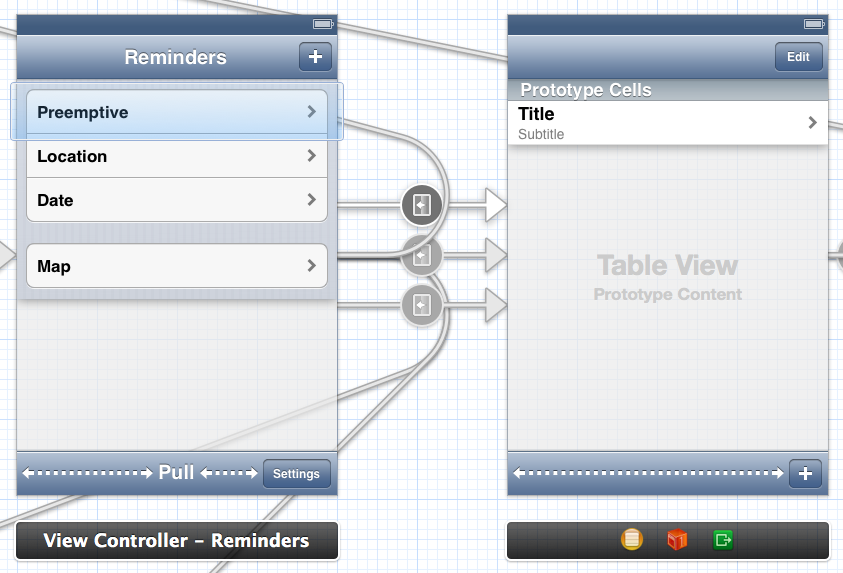
\includegraphics[scale=0.3]{images/reminder-list}
\caption{Storyboard showing segues for different reminder lists}
\label{fig:reminderlists}
\end{figure}

\subsection{Adding Reminders}

An important part of this project was how the user would create and add a reminder. The Calendar app that comes preinstalled on all iOS devices offers a simple and intuitive way to add calendar events. This was used as the inspiration behind adding reminders, and by emulating this offered a familiar way to add reminders if the user has used the Calendar app before. Figure \ref{fig:addreminder} shows the similarities between the two apps.\\

\begin{figure}[H]
\centering
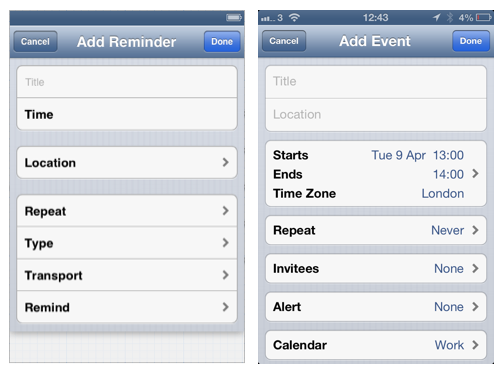
\includegraphics[scale=0.5]{images/add-reminder}
\caption{Comparison of adding a reminder and adding an alert in Calendar.app (right)}
\label{fig:addreminder}
\end{figure}

Although both apps are formatted similarly there are differences between the two. One noticeable difference is how dates are handled. With a calendar event there needs to be a start and end time specified, but with a reminder only the end time is necessary. As only one date is needed for a reminder it is not necessary to display a different view where a date picker is shown as seen in Figure \ref{fig:datepickers}. Instead, when the time field is tapped a modal date picker is shown that uses \texttt{CoreAnimation} in order to display the date picker with an animation similar to when the keyboard is shown.\\

\begin{figure}[H]
\centering
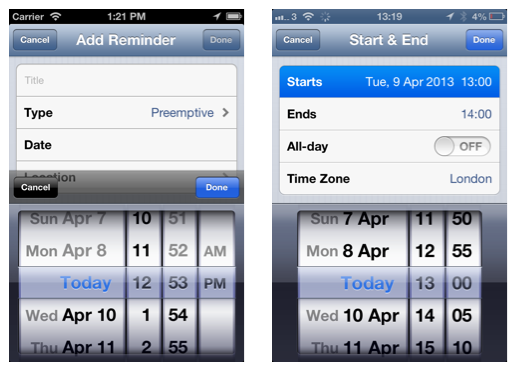
\includegraphics[scale=0.5]{images/date-picker}
\caption{Comparison of Date Pickers in Calendar.app (right)}
\label{fig:datepickers}
\end{figure}

Another difference from Calendar is the location field. Specifying a location when adding an event is essentially represented as a string and holds no geographical information for the given location. When adding a reminder a \texttt{UITabBarController} is displayed to the user as seen in Figure \ref{fig:locationtabbar} providing the ability to add locations from services such as the user's Contacts app and Google Places. These locations have an associated longitude and latitude which can be turned into a \texttt{CLLocation} object and compared with the current location to deliver reminders. 

\begin{figure}[H]
\centering
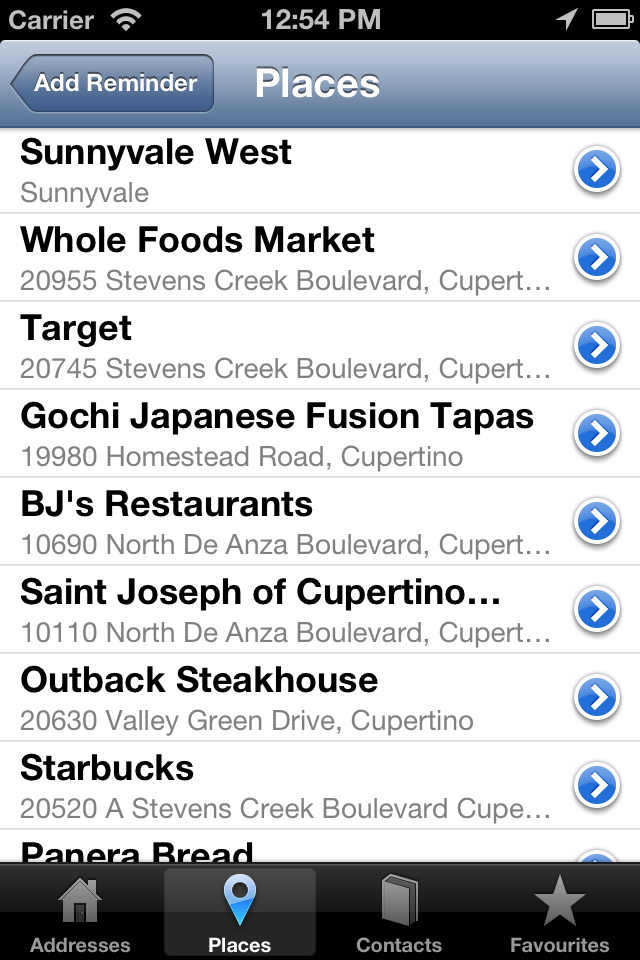
\includegraphics[scale=0.2]{images/location-tabbar}
\caption{Selecting a location using \texttt{UITabBarController}}
\label{fig:locationtabbar}
\end{figure}

\subsubsection{Web Services}

Some of the APIs mentioned in Section \ref{sec:datasources} were used in order to provide multiple data sources when adding reminders. The services used were Google's Places API and their Geocoding API. Foursquare's API was also researched, but upon implementing it in order to sample its functionality it was clear that this service didn't offer data on par with Google's API. This was in part due to the fact that a lot of the data is user sourced and as a result some search results given were unsuitable.\\

The two Google APIs were implemented as separate table views within the locations tab bar. On tapping locations the first view they see in the tab bar is the address search view which is powered by the Geocoding API. The user can search for a place which is then sent as a request to the service and the JSON output is returned. This JSON data is parsed and shown as places in the table. As this view has no data to show until the user searches, the last ten places used as reminders from this service are cached and shown in this table view. The places table view is populated using the Places API. On loading this view, the user is shown places of interest for their current location and using the search bar allows nearby places to be found in a similar manner to the addresses view. In order to ensure good performance throughout the app, threads are used with all network requests as it is important to not block the main thread as this is where the UI code is executed.\\

Initially when searching for a place, an API request was made for each character entered on the keyboard creating an instant search. This feature worked well but both APIs suffer from rate limitations. In order to ensure these API limits were not reached, this functionality was removed and because of this results are only displayed to the user upon pressing the search button on the keyboard.

\subsection{Favourites}
 
When using location reminders there is the possibility of adding a reminder for a place that has previously been used. In order to save the user from having to always search for a place they wish to use regularly a favourites table view has been added to the tab bar. When viewing the details for a button is displayed and dependent on whether the location exists in favourites the button either favourites or un-favourites that location. Once a favourite has been added it is stored in the same way that reminders are stored and is persistent between uses of the app.
 
\section{User Interface}

\subsection{UIAppearance}

The previous chapter talks about using \texttt{UIAppearance} in order to customise the user interface. In order to customise a \texttt{UIAppearance} proxy, UI elements are needed. Adobe Photoshop provided a way to create professional looking elements that could be saved as retina and non-retina images in order to work with all devices. Some of these elements can be seen in Appendix \ref{appendix:appendix1}.

\subsection{Reminders Tray}

During implementation it was identified that it would be useful to be able to show the user what reminders they will be alerted about next. Creating another view controller to show this information would not be an ideal solution as the user only has to tap on a reminder type to be shown all the reminders for that type. Instead a better solution would be to show these reminders on the home screen of the app. By hiding these reminders underneath the app they could be shown to the user through an animation as opposed to segueing to a different view entirely.\\

In order to create this animated reminder tray inspiration was taken from some of the animations already found in iOS, so that the user would be familiar with how the functionality works even if they have not used the app before. The lock-screen found on the iPhone features a camera button that when dragged slides up to reveal the camera app, this is also present when the home button is double tapped and reveals the multitasking tray as shown in Figure .

TODO: add pics here.

In order to implement similar functionality, a button was added to the toolbar on the home screen of the app. This button uses a gesture recogniser in order to know not only when the button is tapped but when it is dragged also. As the button is dragged the view is pushed up the screen revealing underneath the current reminders. In order for the user to identify that they can drag the toolbar the button has been replaces by an image that creates the impression of indentation on the toolbar which leads to the user identifying that it can be dragged. This is also similar to the camera button previously mentioned. On the lockscreen, tapping this camera button causes a bounce animation allowing the user to identify there is something underneath without actually showing the user. By using \texttt{CoreAnimation} this animation war replicated and tapping the toolbar causes the view to move up and down in a similar manner. The reminders tray can be seen in Figure

TODO: add reminder tray pics here.

\section{Testing}

Since the scope and the codebase for this project is relatively large, it is important that the app is thoroughly tested, especially if the app is to be distributed on the App Store. Apple provide a unit testing framework, called \texttt{OCUnit} for testing application logic as well as \texttt{OCMock} which allows that actual app to be tested programatically triggered touches in order to interact with the app. This two methods of testing were only discovered near to the end of this project and as a result not used. Some manual tests were written during the stages of implementing the reminder logic in order to test that it worked correctly. For instance in order to check the priority queue was storing the reminders in the correct order a number of reminders with various dates were added.\\

When a new feature had been implemented the iOS simulator was used in order to quickly check that it functions correctly, but running on the device has been the most reliable way to test the app. As a result a lot of user testing was used.

\subsection{TestFlight}

TestFlight \cite{testflight} provided a way to distribute apps to testers without having to use the App Store meaning early and unfinished builds of the app could be used without submitting an app that would inevitably get rejected from the App Store. TestFlight allows testers to be invited and register their device so that the developer can provision their device in the Apple Dev Center so the app can be signed with a certificate which allows the app to run on the testers device.\\

Testing was carried out by a small group of users on a range of devices such as iPhone 4, iPhone 4S and iPhone 5. It would have been useful to test the performance and UI on an iPhone 3GS, but the simulator was at least able to show what the non retina 3GS screen would look like. TestFlight shows which build of the app that they are running and also provides a way to receive tester feedback from within the app which can be seen in Figure \ref{fig:testflight}. 

\begin{figure}[h!]
\centering
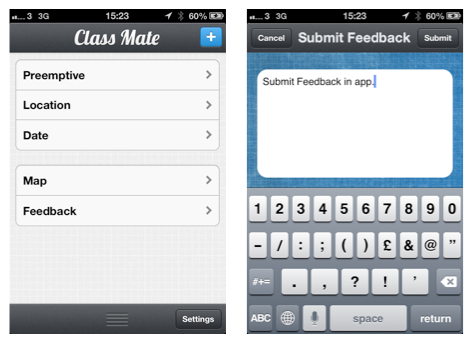
\includegraphics[scale=0.75]{images/testflight}
\label{fig:testflight}
\caption{Submitting feedback within the app}
\end{figure}

\subsection{Crashlytics}

Crashlytics \cite{crashlytics} is a framework that was used in the app in order to receive crash reports. These crash reports provided valuable information for fixing bugs during the testing and is still present in the current version of the app found on the App Store. If a crash is detected by the Crashlytics framework, a crash report is created against the app in order to identify the line of the code where the crash occurred.

TODO: Show figure here

\section{App Store}

Upon reaching a stage of user testing where no major bugs were being found, the app was prepared for distribution on the App Store. 

\subsection{Submitting}

As the app was modified to include the TestFlight framework as well as adding the a feedback button to allow for feedback to submitted, these would need to be removed in order for app to be approved. To get around this, a macro was defined that would check to see if the app was a testing build and if so the code for using the TestFlight framework and showing a feedback button would be executed. Once the app was in a state ready for submission it was archived in order to create the binary that can be downloaded on the App Store.\\

The first step to submitting an app to the App Store is by adding a new app in iTunes Connect. Apple require details about the app, screenshots and icons in order to be able to upload the binary. Once this has been done the app can be validated in order to make sure it contains all the required assets to be submitted. The app was validated and then submitted from Xcode. Once an app has been submitted there are several steps that the app has to pass before it can be downloaded by users on the App Store; 

\begin{description}
\item[Waiting for Upload]As soon as the app is created on iTunes Connect, the review status is waiting for the binary to be uploaded.
\item[Upload Received]Once the binary has been uploaded, this review status should be show for a small amount of time before moving onto the next stage of the process.
\item[Waiting for Review]This status is given when the app is in the queue with other apps to be reviewed and is dependant on how many other apps there. At the time of submitting the average time to enter review was between 6 and 7 days. 
\item[In Review]This is that status given when an Apple reviewer is looking at the app to ensure it conforms with the the strict App Store guidelines \cite{appreview}. If the app does not pass this stage it may be rejected.
\item[Processing for App Store]Upon passing the review stage, the app is readied to be sold it multiple countries.
\item[Ready for Sale]This is the final status of the review process, means the app will automatically roll out to the App Store or be released on the day set if a release date was given.

\end{description}

\subsection{Rejection}

After seven days into the review process the app was marked as metadata rejected. This means that the app has not be rejected in regard to its functionality but the description that would be seen by users downloading the app on the App Store. The reviewer suggested that a disclaimer should be added to the description by including the following; "Continued use of GPS running in the background can dramatically decrease battery life." Once the disclaimer has been added, the app was resubmitted and because only the app metadata was changed and not the app binary, it was given the status 'In Review' shortly after.

\subsection{Approval}

The app was 'Processing for App Store' two days after being resubmitted and shortly after became 'Ready for Sale'. Since the app had been set to release the day before the project presentation, it did not suffer from the delay commonly associated with releasing an app as soon as it is approved.

\chapter{Project Management}

\section{Software Development Methodology}

The methodology used in the development of this software project was incremental development. According to Raymond Lewallen \cite{raylewallen} the incremental approach is where working software is produced during the first iteration, and future iterations build on that software. This has been the case for this project, by adding small amounts of functionality to make a working app in early iterations, and continued iterating until the app was ready to be distributed on the App Store. One of the benefits of an incremental approach is ease of testing as their is less to test in early iterations, and it later iterations much of the software has already been tested.\\

By user testing the app, various bugs were found during the testing phase. Here the incremental approach was used as for each bug report or crash report received an iteration was made on the software in order to fix that bug or crash.

\section{Code Management}

With large software projects it is very important to manage code efficiently. For this project Git was used in order to manage code versions. One advantage of using Git is that Xcode features built in support meaning that it is easy to see the state of the repository by showing the current versioning of classes and other files from within the IDE. Another reason for employing Git is that it provides an easy way to maintain branches of the codebase. For instance a branch might be created for a new feature to be added. If that feature works well if can be merged into the master branch, but if it does not work well there is no need to add it to the master branch and the code from the master has not been affected. GitHub \cite{github} was used to provide a central repository so that the codebase could be cloned and development could take place on multiple machines.\\ 

One problem with using Git has been with storyboards, as these do not work well with versioning and as a result apps developed as part of a team using a version control system in order to collaborate would benefit from creating user interfaces only using code in order to avoid the problem of multiple people working on the same storyboard.

\chapter{Conclusion}

\section{Project Evaluation}

In order to evaluate the project, we have to look back to see if it meets its original aims as well as seeing how closely it follows the project specification. The two main aims of this project were to implement the reminder functionality and to create a shipping app that is available for users to download from the Apple App Store. Both of these aims have been achieved, as the app is available to download on the App Store \cite{classmate} and from user testing established that the reminder functionality works as stated.

During the project a specification was created to outline both the functional and non functional requirements of this project. In order to evaluate this project fully it is important to compare the final version of the app to this specification. In terms of functional requirements, the app met the majority outlined in the specification, as the reminder functionality works for all types of reminders. \texttt{CoreLocation} is used in order to provide location services for the app but does only use location when necessary in order to conserve battery. \texttt{MapKit} was used in order to display a users reminders on a map and the user is able to add a reminder both quickly and easily. However, one functional requirement was not met - the  significant location change service was not used when the app was in the background due to constraints as specified in Section \ref{sec:significantlocation}.\\

In terms of non-functional requirements, again the majority of them were met. As specified the app was created using the Objective-C language. In terms of usability the app used standard iOS navigation paradigms and buttons throughout the app featured recognisable icons as well as using a custom user interface through \texttt{UIAppearance}. The performance requirements were that battery usage should be kept at a minimum and for the most part this was true although as previously stated low power location services could not be used and as a result more battery usage does take place than initially desired. The app is also reliable as user testing helped ensure the stability of reminders and the persistence of them between app uses. The project specification outlines that no personal data must be stored or transferred. This requirement was met as only the users current location is sent to the APIs used in the project, but always sent securely over SSL. The final requirement - portability was not fully achieved as all iOS devices can provide location services but the app was limited to devices that have GPS available.

\section{Limitations}

Although the app meets its main aims, there are limitations in the current iteration of the app. The main limitation is the fact that for preemptive reminders only the first reminder in the priority queue is processed, ideally all reminders should be checked but due to the limitations of the device this is not plausible as many API requests would have to be made resulting in more battery drainage than is already occurring from usage of the location services. As a result of only checking the first reminder it might be the case that when multiple preemptive reminders are added, even though when both reminders were added there was enough time to get to each of them, that upon reaching the one destination they are too far away to then reach the second destination on time and will not be told until they are alerted for the first reminder.\\

Due to the fact that the app makes API requests in the background to calculate when the user needs to be alerted, an internet connection is required. If the users device loses signal cannot make the API requests needed, the original method for calculating the time away from the destination is used, but as that does not have the same level of accuracy as compared to using Google's API the reminder may be fired even though it is not yet necessary. The omission of an edit button is another limitation of the app and as a result requires users to delete a reminder and re-add the updated reminder.

\section{Future Enhancements}

Since the scope for this projects there are numerous enhancements and continuations that could be made on this project. One enhancement could be the inclusion of URL schemes \cite{urlscheme}. URL schemes are used throughout iOS in order to allow apps to communicate with each other and by implementing a URL scheme it would allow other apps to add reminders without having to implement any of the functionality themselves. For example an app where you can make a reservation at a restaurant could then call the URL scheme to add a reminder to that restaurant. Another possible enhancement is to widen the number of devices and platforms the app is available for, initially a possible extension was to create an iPad interface for the app, but since the app require GPS for its core functionality there seemed no point (change this). Porting the app to Android and other platforms would be a possibility especially consider there are tools available to automatically convert Objective-C logic code to Java \cite{objc2j} meaning only the user interface would have to be recreated for this other platform.

\section{Overview}

During this project I had to learn about various aspects of the Objective-C language which I had no prior experience with, such as \texttt{CoreLocation}, \texttt{MapKit} and \texttt{CoreAnimation}. As a result I feel more confident as an Objective-C programmer and can carry these newly learnt skills over to the next project I undertake. 

Although happy with the overall state of the project, I feel I could have performed better as although the reminder functionality works as stated the code base isn't as clean as I would like it to be. One of the aims was to create this functionality in a way so that other apps could use it in the same way frameworks such as \texttt{CoreLocation} are used. Due to the time constraints for this project this was not fully achieved and during implementation of the app methods had to be added to the reminder manager that were needed but not originally considered. Also due to time constraints no extensions were added to the project although there was scope for many extensions.\\

I however am happy with several parts of the project. Firstly I am proud of the fact that I was able to ship the app and have it approved to be included on the App Store. I am also really happy with how my user interface looks as a lot of effort went it to creating it and have been told that it looks like a professionally made app. It was also a challenge in order to get the preemptive reminder functionality working considering the limitations and constraints of the device it is used on and I am pleased with the results.

Overall I feel that the project can be considered a success as the majority of the aims for this project were completed and the finalised app is something that I can be proud of.

\newpage
\printbibliography
\newpage

\appendix
\section{User Interface Elements}\label{appendix:appendix1}
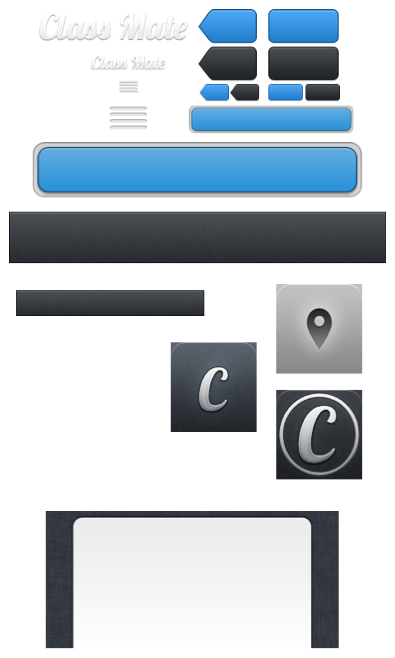
\includegraphics{images/ui-elements}

\section{Storyboard}\label{appendix:storyboard}
\centering{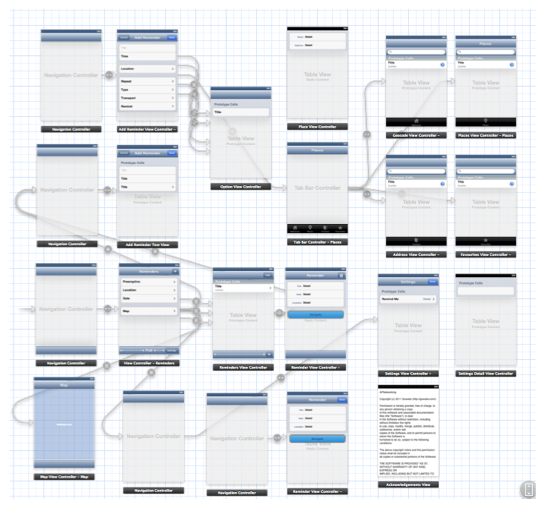
\includegraphics[scale=0.9]{images/storyboard}}

\section{App}\label{appendix:app}

\includegraphics{images/class-mate}

\section{User Guide}

\end{document}
